\documentclass[letterpaper,11pt]{amsart}

\usepackage{amscd,amssymb,amsfonts,amsmath,amsthm,color}
\usepackage{enumerate}
\usepackage{listings}
\usepackage{courier}
\usepackage{graphicx}
\usepackage{scrextend}

\usepackage{calc}
\newsavebox\CBox
\newcommand\hcancel[2][0.5pt]{%
  \ifmmode\sbox\CBox{$#2$}\else\sbox\CBox{#2}\fi%
  \makebox[0pt][l]{\usebox\CBox}%  
  \rule[0.5\ht\CBox-#1/2]{\wd\CBox}{#1}}


\lstset{frame=lrbt,xleftmargin=\fboxsep,xrightmargin=-\fboxsep,colframe=gray}


\lstset{basicstyle=\ttfamily\footnotesize,breaklines=true}


%%%%%%%%%%%%%%%%%%%%%%%%%%%%%%%%%%%%%%%%%%%%%%%%%%%%%%%%%%%%
% margins and style
\pagestyle{plain}
\setlength{\evensidemargin}{0.25in}
\setlength{\oddsidemargin}{0.25in}
\setlength{\textwidth}{6.0in}
\setlength{\topmargin}{0.0in}
\setlength{\textheight}{8.5in}
\setlength{\headheight}{0in}
\setlength{\parskip}{1.5mm}

\linespread{1.2}
\usepackage{color}
\definecolor{gray}{rgb}{0.3,0.3,0.3}



%%%%%%%%%%%%%%%%%%%%%%%%%%%%%%%%%%%%%%%%%%%%%%%%%%%%%%%%%%%%
% theorems and all 
\theoremstyle{plain}
\newtheorem{theorem}{Theorem}[section]
\newtheorem{lemma}[theorem]{Lemma}
\newtheorem{proposition}[theorem]{Proposition}
\newtheorem{corollary}[theorem]{Corollary}

\theoremstyle{definition}
\newtheorem{definition}[theorem]{Definition}
\newtheorem{remark}[theorem]{Remark}

%%%%%%%%%%%%%%%%%%%%%%%%%%%%%%%%%%%%%%%%%%%%%%%%%%%%%%%%%%%%
% renewed commands: t, to, d , c, H

%%%%%%%%%%%%%%%%%%%%%%%%%%%%%%%%%%%%%%%%%%%%%%%%%%%%%%%%%%%%
% Shortcuts for tex commands

\newcommand{\nc}{\newcommand}
\newcommand{\rc}{\renewcommand}
\nc{\mc}{\mathcal}
\rc{\t}{\text}
\nc{\loccit}{\emph{loc. cit. }}
\nc\pf{\noindent Proof: }
%%%%%%%%%%%%%%%%%%%%%%%%%%%%%%%%%%%%%%%%%%%%%%%%%%%%%%%%%%%%
% Operators, functions etc
\nc{\Hom}{\t{Hom}}
\nc{\tot}{\t{tot}}
\nc{\dual}{^{\vee}}
\nc{\op}[1]{\operatorname{#1}}
\nc{\coh}{\t{coh}}
\nc{\iso}{\cong}
\rc{\d}{\operatorname{d}}
\nc{\Id}{\operatorname{Id}}
\nc{\dgmod}{\operatorname{dg-mod}}
\newcommand{\hdot}{^{\raisebox{0pt}{\text{\circle*{2}}}}}
\nc{\compose}{\circ}
\nc{\sheafsym}{\mathcal{S}\t{ym}}
\nc{\rend}{\operatorname{REnd}}
\nc{\rhom}{\operatorname{RHom}}
\nc{\sheafrend}{\mathcal{R}\mc{E}\t{\emph{nd}}}
\nc{\sheafrhom}{\mathcal{R}\mc{H}\t{\emph{om}}}
\nc{\sheafhom}{\mathcal{H}\t{om}}
\nc{\exterior}{{\textstyle\bigwedge\nolimits}}
\nc{\ex}{\exterior}
\nc{\cok}{\operatorname{Coker}}
\rc{\ker}{\operatorname{Ker}}
\nc{\im}{\operatorname{Im}}

%tensor product
\nc{\Lotimes}{{\overset{L}{\otimes}}}
%%%%%%%%%%%%%%%%%%%%%%%%%%%%%%%%%%%%%%%%%%%%%%%%%%%%%%%%%%%%
% Arrows and signs
\rc{\to}{\rightarrow}
\nc{\ot}{\leftarrow}
\nc\xto[1]{\xrightarrow{#1}}
\nc{\too}{\longrightarrow}
\nc{\oot}{\longleftarrow}
\nc{\into}{\hookrightarrow}
\nc{\mapsinto}{\hookrightarrow}
%%%%%%%%%%%%%%%%%%%%%%%%%%%%%%%%%%%%%%%%%%%%%%%%%%%%%%%%%%%%
% Categories
\nc{\D}{\operatorname{D}}
\nc{\Dsg}{\D_{{sg}}}
\nc{\Db}{\D^{{b}}}
\nc{\Dbgr}{\Db_{{gr}}}
\nc{\Dgr}{\D_{{gr}}}
\nc{\Dsggr}{\Dsg^{{gr}}}
\nc{\Cgr}{\operatorname{C}_{{gr}}}
\nc{\cCgr}{\cC_{gr}}
\nc{\cDgr}{\cD_{gr}}
\nc{\cDsggr}{\cD_{gr}^{sg}}
\nc{\cDbgr}{\cD_{gr}^{b}}
\nc{\cDsg}{\cD_{sg}}
\nc{\cDb}{\cD^{b}}
\rc{\H}{\operatorname{H}}

%%%%%%%%%%%%%%%%%%%%%%%%%%%%%%%%%%%%%%%%%%%%%%%%%%%%%%%%%%%%
% Nice letters
% cals
\nc{\cA}{\mc{A}}\nc{\cB}{\mc{B}}\nc{\cC}{\mc{C}}\nc{\cD}{\mc{D}}\nc{\cE}{\mc{E}}\nc{\cF}{\mc{F}}\nc{\cG}{\mc{G}}\nc{\cH}{\mc{H}}\nc{\cI}{\mc{I}}\nc{\cJ}{\mc{J}}\nc{\cK}{\mc{K}}\nc{\cL}{\mc{L}}\nc{\cM}{\mc{M}}\nc{\cN}{\mc{N}}\nc{\cO}{\mc{O}}\nc{\cP}{\mc{P}}\nc{\cQ}{\mc{Q}}\nc{\cR}{\mc{R}}\nc{\cS}{\mc{S}}\nc{\cT}{\mc{T}}\nc{\cU}{\mc{U}}\nc{\cV}{\mc{V}}\nc{\cW}{\mc{W}}\nc{\cX}{\mc{X}}\nc{\cY}{\mc{Y}}\nc{\cZ}{\mc{Z}}
% bbs
\nc{\PP}{\mathbb{P}}
\nc{\CC}{\mathbb{C}}
\nc{\ZZ}{\mathbb{Z}}
\nc{\HH}{\mathbb{H}}
\nc{\NN}{\mathbb{N}}
\nc{\QQ}{\mathbb{Q}}
\nc{\RR}{\mathbb{R}}


\nc{\code}[1]{{\texttt{#1}}}
\nc{\mcode}[1]{{\text{\texttt{#1}}}}



%%%%%%%%%%%%%%%%%%%%%%%%%%%%%%%%%%%%%%%%%%%%%%%%%%%%%%%%%%%%
% other useful commands
\let\oldmarginpar\marginpar
\renewcommand\marginpar[1]{\-\oldmarginpar[\raggedleft\footnotesize #1]%
{\raggedright\footnotesize #1}}
\nc\note[1]{\marginpar{#1}}

%%%%%%%%%%%%%%%%%%%%%%%%%%%%%%%%%%%%%%%%%%%%%%%%%%%%%%%%%%%%
%%%%%%%%%%%%%%%%%%%%%%%%%%%%%%%%%%%%%%%%%%%%%%%%%%%%%%%%%%%%
%%%%%%%%%%%%%%%%%%%%%%%%%%%%%%%%%%%%%%%%%%%%%%%%%%%%%%%%%%%%
%%%%%%%%%%%%%%%%%%%%%%%%%%%%%%%%%%%%%%%%%%%%%%%%%%%%%%%%%%%%
%%%%%%%%%%%%%%%%%%%%%%%%%%%%%%%%%%%%%%%%%%%%%%%%%%%%%%%%%%%%

\title{Homework 5}
\date{}
\begin{document}
\maketitle
\begin{center}
  \emph{Due Thursday, Feb 23, at 11pm}
  \vspace{0.3in}
  \end{center}


\noindent Please enter your answers into a Jupyter notebook and submit by the deadline via canvas. 

\subsection*{A Class for Polynomials} Design a class called \code{Polynomial} for polynomials in one variable. You should use a list to store the coefficients of the polynomial. I should be able to do the following:
\begin{itemize}
  \item Initialize my polynomial using a list of its coefficients: e.g. \code{p = Polynomial([1.0, 2.0, 3.0])}
  \item Print my polynomial: e.g. \code{print(p)} for the \code{p} above should give: \code{1.0x\string^0 + 2.0x\string^1 + 3.0x\string^2}. You should implement \code{\_\_repr\_\_(self)} in your class for this, which should return a string. (optional: make sure you print negative coefficients correctly) 
  \item Add polynomials to get a new polynomial. (implement \code{\_\_add\_\_(self, other)} in your class for this, it should return a new polynomial)
  \item Evaluate the polynomial at a value x by running \code{p.eval(x)}. e.g. for the above polynomial, \code{p.eval(2.0)} should return \code{17.0}.
\end{itemize}

\subsection*{Complex Numbers in Python} 

Complex numbers are numbers of the form $a + bi$ where $a,b \in \RR$. The number $i = \sqrt{1}$ is the formal square root of $1$, which we pretend exists. So we have $i^2 = -1$, and $i^3 = -i$ and $i^4 = 1$. The rules for addition and multiplication of complex numbers follow the usual algebraic rules. For example:
$$(2 + 3i) + (1 + 5i) = 3 + 8i$$
$$(2 + 3i)(1 + 5i) = 2 + 10i + 3i + 15i^2 = 2 + 13i - 15 = -13 + 13i $$

We can represent complex numbers on the plane as follows:

\begin{center}
\noindent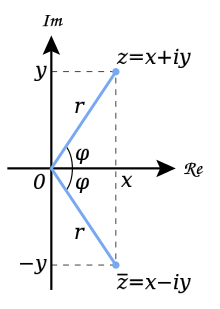
\includegraphics[width=1.6in]{complex_nums.png}
\end{center}

Here the number $z = x + yi$ is represented on the plane. $\bar{z} = x - yi$ is called the complex conjugate of $z$. We have

$$ z\bar{z} = (x+yi)(x-yi) = x^2 -xyi + yxi -y^2i^2 = x^2 + y^2$$

So the norm (i.e. distance to the origin) of a complex number $z$ is $|z| = \sqrt{x^2+y^2} = \sqrt{z\bar{z}}$. 

The angle $\varphi$ between $z$ and the $x$ axis is called the phase of $z$. If $z$ has phase $\varphi$, then $z = |z|(\cos(\varphi) + i \sin(\varphi))$.

We have the formula
$$e^{i\theta} = \cos{\theta} + i \sin{\theta}$$

So, for every complex number $z$, we have:

$$z = |z|e^{i\op{phase(z)}}$$

This leads to the famous formula:
$$e^{i\pi} = -1$$
(math-tattoo anyone?)

Remark:

$$z_1z_2 = |z_1|e^{i\op{phase(z_1)}}|z_2|e^{i\op{phase(z_2)}} = |z_1||z_2| e^{i(\op{phase}(z_1) + \op{phase}(z_2))}$$

So when you multiply two complex numbers, you multiply the norms, and you add up the angles. 

In Python, complex numbers are represented by expressions like \code{2+3j}. Here, it is important that there is no space between the \code{3} and the \code{j}. 

If we set \code{z = 3 + 4j} then we can use \code{z.real} and \code{z.complex} to access the real and imaginary parts of \code{z}, namely \code{3} and \code{4} in this case. 

\begin{itemize}
  \item Write a function norm(z) that returns the norm of a complex number $z$. (as a float. e.g. (\code{norm(3+4j)} should return \code{5.0})) 
  \item Understand the code below, and then complete the function below to produce the pictures shown.
    
\end{itemize}

\begin{lstlisting}[language=python]
import libhw01 as libhw
from cmath import phase
import math
from math import pi

# draws a picture for a function f: Complex -> Reals
def drawComplexFunction(f, imsize=300):
    g = lambda x,y: f(x+y*1j)
    libhw.drawfunction(g, imsize=imsize)

def norm(z):
    return math.sqrt(z.real * z.real + z.imag * z.imag)

def f_one(z):
    if # . . . something about phase(z) . . . 
        return 1.0
    return 0.0

def f_two(z):
    # modify f_one, hint: take a power of z
    return 0.0

# modify this function to get the one in the third picture 
def f_three(z):
    return math.sin(phase(z) + norm(z))

def f_four(z):
    # combine the ideas of f_two and f_three
    # and then figure out a trick to shift the picture slightly in one direction

drawComplexFunction(f_one)
drawComplexFunction(f_two)
drawComplexFunction(f_three)
drawComplexFunction(f_four)
\end{lstlisting}

\begin{center}
\noindent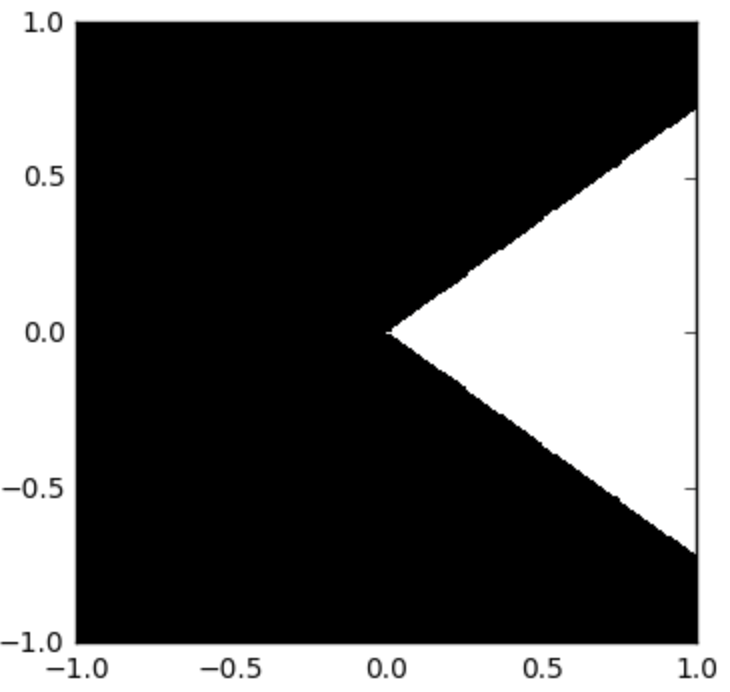
\includegraphics[width=2.6in]{im1.png}
\noindent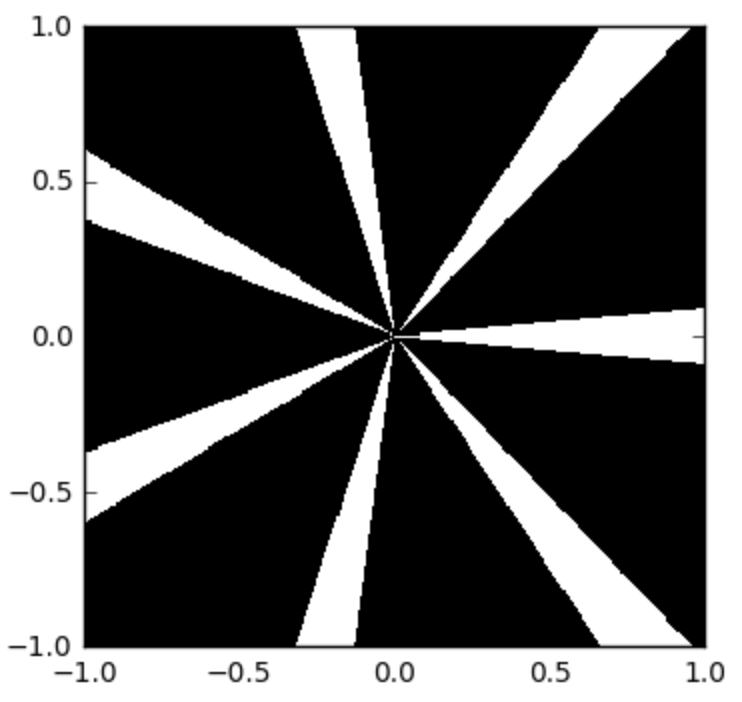
\includegraphics[width=2.6in]{im2.png}
\noindent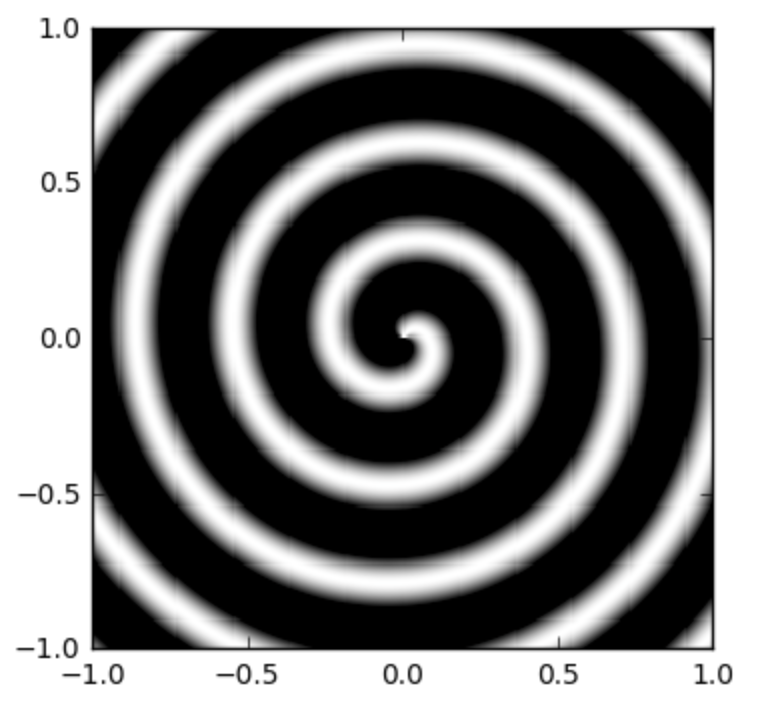
\includegraphics[width=2.6in]{im3.png}
\noindent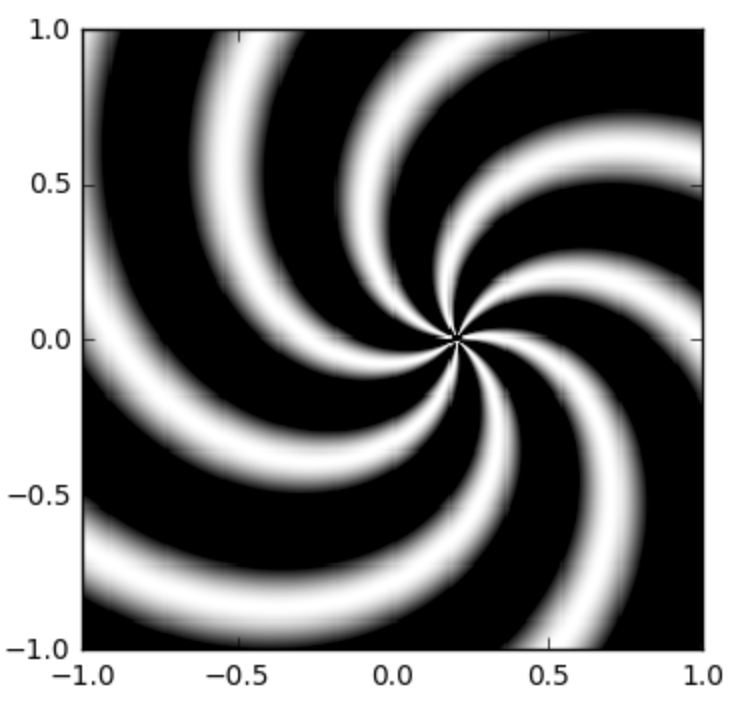
\includegraphics[width=2.6in]{im4b.png}
\end{center}

\subsection*{The Julia Set in the Complex Plane} 

The Julia set $J_c$ is defined as follows. Let $f(z) = z^2 + c$. Apply $f$ repeatedly to a complex number $z$, i.e. take $f(z)$, $f(f(z))$. $f(f(f(z)))$, \dots This is an example of a \emph{dynamical system}. 

As you do this, a typical point will lead to expenential growth as you keep squaring and adding $c$ (i.e. the norm grows exponentially) . The Julia set $J_c$ is the set of points which don't grow exponentially when you do this.  

To compute the Julia set, we will do the following: we will start with $z$ and compute  $f(z)$, $f(f(z))$. $f(f(f(z)))$,\dots $f^k(z)$ for a fixed $k$, e.g. $k = 100$. If the result has norm $|f^k(z)| < 2$, we will assume $z$ is in the Julia set. 

To get a little nicer a picture of the Julia set, we will do the following:  $|f^k(z)| < 2$ after $k$ iterations, the pixel will have white value (i.e. your function should output 1), but if $|f^i(z)| > 2$ at the $i$th iteration and not before, then the value will be $i/k$, so that it appears more white the closer it is to the actual Julia set.

\begin{itemize}
  \item Complete the code below to draw the Julia set for $c = 0.28 + 0.008i$.
  \item Find another $c$ which gives an interesting picture (you will have to do this by trial and error).
\end{itemize}


\begin{lstlisting}[language=python]
def julia(c,z):
  k = 100
  # in a loop, compute f^i(z) and see when it moved out of the circle of radius 2
  # when it leaves, return i/k

def my_julia(z):
    return julia(0.28 + 0.008j, z)

drawComplexFunction(my_julia, imsize=600)    # imsize = 600 for a little better resolution
\end{lstlisting}

\subsection*{The Mandelbrot Fractal}

Which $c$'s give interesting Julia sets $J_c$? One way to analyze that is the following question: for which $c$'s will the sequence $f(0), f(f(0)), \dots, f^k(0),\dots$ not grow exponentially? If we draw the answer to this, we get the Mandelbrot fractal. i.e. the Mandelbrot fractal is the set of points in the complex plane for which  $f(0), f(f(0)), \dots, f^k(0),\dots$ does not grow exponentially.

\begin{itemize}
  \item Complete the code below to draw the Mandelbrot fractal. 
\end{itemize}


\begin{lstlisting}[language=python]
def mandel(c):
    k = 100
    # . . . should return 1.0 if c is in the Mandelbrot set, and 0.0 otherwise . . . 

drawComplexFunction(mandel)
\end{lstlisting}

For values $c$ closer to the edge of the Mandelbrot set, you get the most interesting Julia sets $J_c$. Using this, you can explore more nice values of $c$ for the previous question (optional). 

\subsection*{Zooming in/out}

We drew these fractals but we would like to frame them nicely and/or zoom into them. At the moment, \code{drawComplexFunction(mandel)
} has the top left corner at $-1 + i$ and the bottom-right at $1 - i$. Write a function \code{reframe(f, z\_top\_left, z\_bottom\_right)} which takes a function $f: \mathbb{C} \to \RR$ and zooms into the square whose top left corner is \code{z\_top\_left} and and bottom-right corner is $\code{z\_bottom\_right}$

For example \code{drawComplexFunction(reframe(f\_four, 0.2 - 0.1j, 0.6 - 0.5j))} should give the picture on the right. 
\begin{center}
\noindent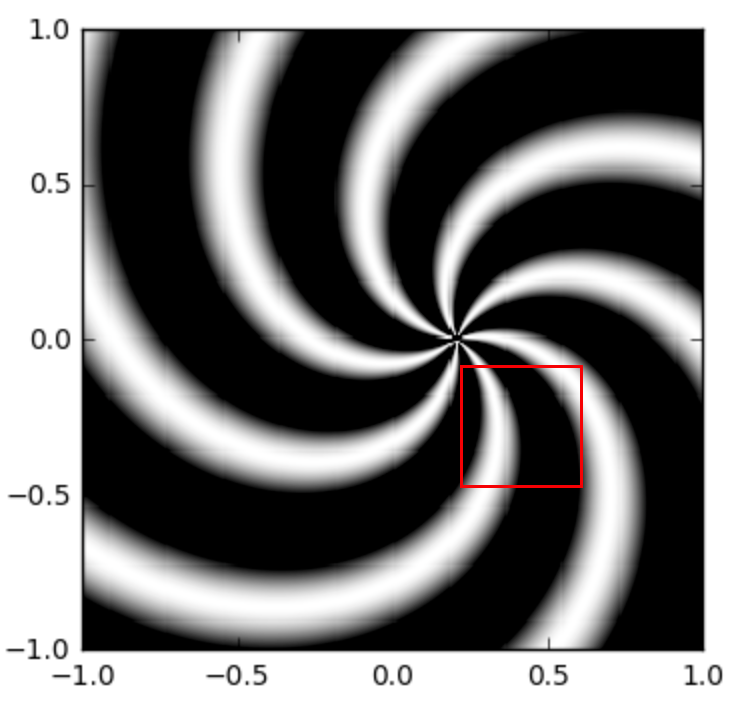
\includegraphics[width=2.6in]{im5_prezoom.png}
\noindent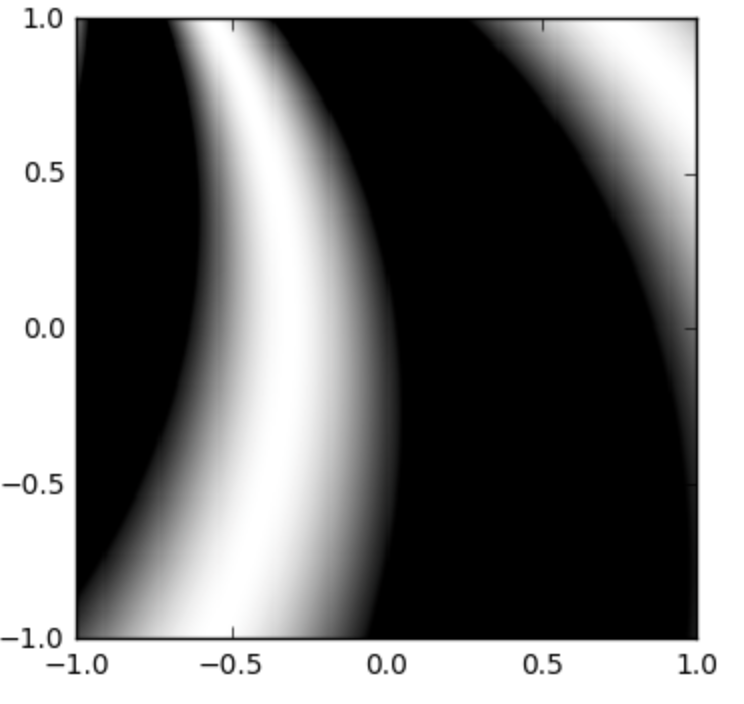
\includegraphics[width=2.6in]{im5_zoomed.png}
\end{center}

\begin{lstlisting}[language=python]
def reframe(f, z_1, z_2):
    def g(z):
        new_z = ???
        return f( new_z )
    return g
\end{lstlisting}

Hint: There are two ways to do this. The first is to get the real and imaginary parts and solve it as a problem for functions $\RR^{2} \to \RR$. The other, more difficult way is to solve the problem for for real numbers and intervals and then generalize to complex numbers.

\begin{itemize}
  \item Use the reframe function you wrote to zoom in (a lot, e.g. 100x, i.e. your top left and bottom right should differ by a complex number of norm around 0.01) to a nice looking part of the Mandelbrot or Julia fractals (you may need to increase $k$ to get enough detail). 
\end{itemize}






\end{document}
%%%%%%%%%%%%%%%%%%%%%%%%%%%%%%%%%%%%%%%%%%%%%%%%%%%%%%%%%%%%






